\section{Objektorientierte Analyse}\label{analyse}
Im Zuge des Kapitels Analyse wird der Prototyp und das verwendete SAP UI5 Framework analysiert und die Ergebnisse in Form von Diagrammen gezeigt und beschrieben. Beginnend werden die Kombinationsmöglichkeiten zwischen den einzelnen Bibliotheken des SAP UI5 Frameworks aufgezeigt. Im Anschluss kommt eine Verdeutlichung eines Nachrichtenflusses innerhalb der SAP UI5 Applikation.

\subsection{Bibliotheken Beziehungen}
Im Zuge der Analyse des SAP UI5 Frameworks wurde zu erst offengelegt wie die einzelnen Bibliotheken innerhalb des Frameworks mit einander kombinierbar sind. Dadurch konnte festgestellt werden, dass einige Bibliotheken zu Gruppen zusammen gefasst werden können und zwei Bibliotheken außen vor liegen. Das wäre zum Einen die Bibliothek \texttt{sap.viz}. Mit ihr wird eine Charting Bibliothek bereit gestellt, die sich mit allen anderen Bibliotheken verwenden lässt. Und zum Anderen die Bibliothek \texttt{sap.ui.inbox}, welche eine fertige Inbox darstellt um sie in Applikationen einzubinden. Die Bibliotheken \texttt{sap.ui.core}, \texttt{sap.ui.layout} und \texttt{sap.ui.unified} lassen sich klar als Kernbibliotheken einordnen. Sie stellen das Grundgerüst des Frameworks. Dann gibt es noch eine Gruppe von Bibliotheken die Controls bereitstellen die eher an die Bedürfnisse einer Desktop Applikation geknüpft sind. Die letzte Gruppe beinhaltet Bibliotheken für Mobile Controls. Sämtliche Mobile Controls funktionieren auch in einer Desktop Applikation, sie sind jedoch für die Anzeige auf mobilen Endgeräten optimiert. Mit Abbildung \ref{fig:sapui5libconnections} sollen diese Gruppen und Beziehungen dargestellt werden.

\vspace{1em}
\begin{figure}[htb]
  \centering
  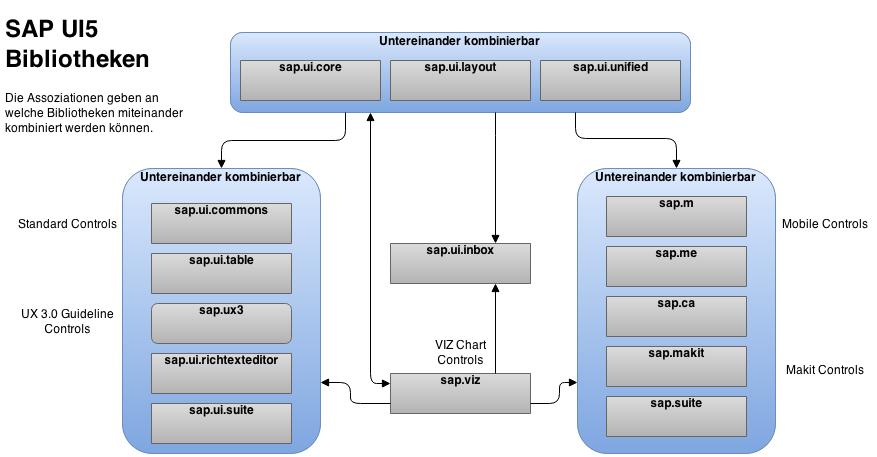
\includegraphics[width=0.95\linewidth]{abb/sapui5_lib_connections}
  \caption[Klassendiagramm: SAP UI5 Bibliotheken Kombinationen]{Klassendiagramm: SAP UI5 Bibliotheken Kombinationen}
  \label{fig:sapui5libconnections}
\end{figure}

\newpage
\subsection{Modularität}
Durch die stringente Verwendung des MVC-Musters können Templates entwickelt werden. Mit diesen Templates lassen sich beispielsweise komplette Geschäftsprozesse abbilden. Geschäftslogik und Präsentation leben in ihrem eigenen Model-View-Controller Verbund. Dadurch kann man sie in den verschiedensten Applikationen wieder verwenden. Der Wartungsaufwand für eine komplexe Applikation lässt sich so verringern. Neben dem MVC-Muster kommt eine zusätzlich Trennung der Präsentationsschicht zu Tragen. Die Struktur wird in JavaScript oder XML definiert, wohingegen die Optik mit CSS beschrieben wird. Dadurch können die Templates schnell und ohne große Hindernisse an ein Corporate Design angepasst werden. Abbildung \ref{fig:sapui5mvctemplates} zeigt diesen denkbaren Einsatz von fertigen UI Templates.

\vspace{1em}
\begin{figure}[htb]
  \centering
  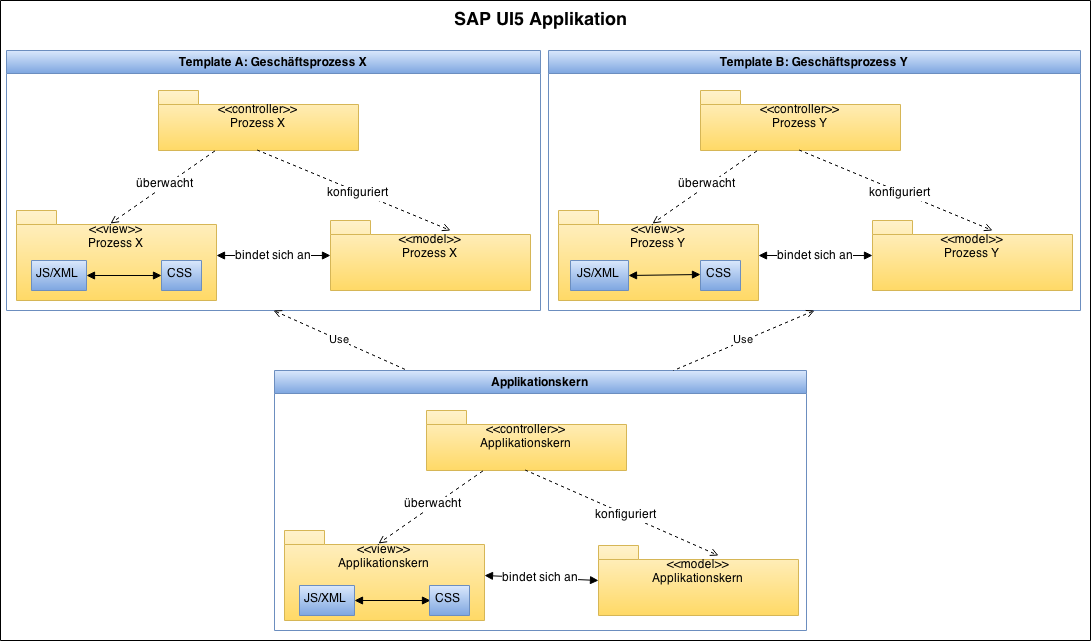
\includegraphics[width=1\linewidth,angle=90]{abb/sapui5_mvc_templates}
  \caption[Paketdiagramm: MVC-Templates innerhalb einer SAP UI5 Applikation]{Paketdiagramm: MVC-Templates innerhalb einer SAP UI5 Applikation}
  \label{fig:sapui5mvctemplates}
\end{figure}

\newpage
\subsection{User Interface Kaskade}
Um ein besseres Verständnis der UI Aufruffolge zu bekommen wurde ein Sequenzdiagramm angefertigt. Mit diesem Diagramm wurde der Aufruf eines Listeneintrags auf der Hauptseite abgebildet. Dieser Klick verursacht die Applikation dazu die ID und den Datenkontext des Eintrags über den Controller an die Detailseite weiterzugeben und dort die vorhandenen Informationen darzustellen. Auf dem Weg dorthin übernimmt der Controller der Detailseite die Aufgabe die beiden verfügbaren Charts zu konfigurieren. Dabei werden die Beschriftung und die Datenherkunft festgelegt.

\vspace{1em}
\begin{figure}[htb]
  \centering
  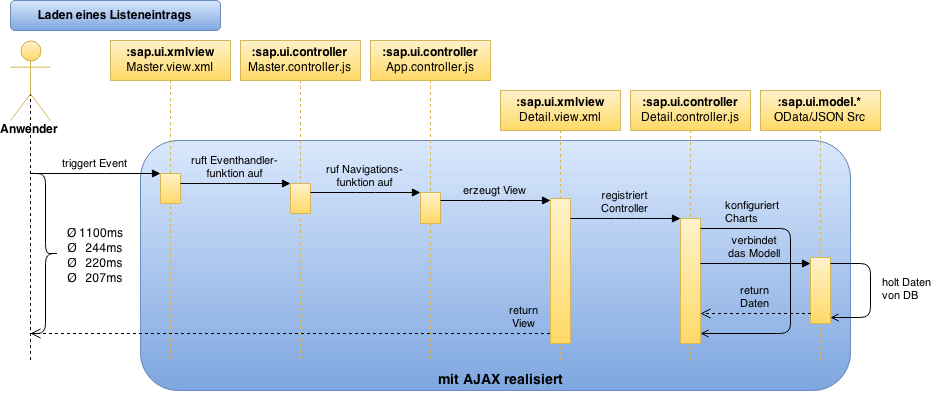
\includegraphics[width=1.05\linewidth,angle=90]{abb/sapui5_load_list_entry}
  \caption[Sequenzdiagramm: Laden eines Listeneintrags]{Sequenzdiagramm: Laden eines Listeneintrags}
  \label{fig:sapui5loadlistentry}
\end{figure}

\paragraph{Zeitmessung}$\;$ \\
Um das Sequenzdiagramm mit Meta-Informationen anzureichern wurde eine Zeitmessung vorgenommen. Es wurden 4 Werte gemessen. Alle Versuche wurden mit deaktiviertem Browser Cache gemessen. Die erste Messgröße ist die Dauer vom öffnen bis zur fertig geladenen Seite. Danach wurden 3 Einträge aus der Liste gewählt und jeweils gewartet bis die Detailseite vollständig geladen und das Chart aufgebaut war. Aus den erhobenen Versuchswerten ist noch der arithmetische Durchschnitt gebildet worden. Alle Ergebnisse sind in Tabelle \ref{tab:uiloading} aufgeführt.

\vspace{1em}
\begin{center}
  \begin{tabular}{ | c | c | c | c | c | c | }
    \hline
    \textbf{Versuch}
    & \textbf{Seite} & \textbf{Detail} & \textbf{1. Klick} & \textbf{2. Klick} & \textbf{3. Klick}\\
    \hline \hline
    1 & 756ms & 742ms & 382ms & 227ms & 205ms\\
    \hline
    2 & 804ms & 877ms & 515ms & 214ms & 205ms\\
    \hline
    3 & 691ms & 888ms & 390ms & 219ms & 200ms\\
    \hline
    4 & 774ms & 743ms & 384ms & 229ms & 200ms\\
    \hline
    5 & 696ms & 736ms & 387ms & 282ms & 206ms\\
    \hline
    6 & 727ms & 818ms & 382ms & 215ms & 211ms\\
    \hline
    7 & 882ms & 620ms & 378ms & 221ms & 281ms\\
    \hline
    8 & 748ms & 729ms & 391ms & 299ms & 210ms\\
    \hline
    9 & 698ms & 729ms & 383ms & 241ms & 276ms\\
    \hline
    10 & 684ms & 881ms & 389ms & 213ms & 198ms\\
    \hline \hline
    \textbf{\O} & \textbf{746ms} & \textbf{776ms} & \textbf{398ms} & \textbf{236ms} & \textbf{199ms}\\
    \hline
  \end{tabular}
\captionof{table}{Chrome Browser UI Ladezeiten}
\label{tab:uiloading}
\end{center}

Aus diesen Ergebnissen lässt sich ablesen, dass das UI beim ersten Aufruf der Applikation im Durchschnitt in unter einer Sekunde geladen und für den Anwender sichtbar ist. Dabei ist zu sagen, dass sich selbe Versuchsreihe mit aktiviertem Browser Cache nur minimal bei den Ergebnissen unterscheidet als mit deaktiviertem Browser Cache. Erfolgt dann der Klick vom Anwender auf einen Listeneintrag wird von der Applikation die Detailseite geladen. Dies geschieht durchschnittlich in 776 Millisekunden. Bei dieser Auswahl eines ersten Listeneintrags, ganz gleich seiner Position innerhalb der Liste, dauert das Laden der Informationen innerhalb der Detailseite im Durchschnitt 398 Millisekunden. Das Laden der Daten und Refreshen der Detailseite dauerten beim zweiten und dritten Listeneintrag im Durchschnitt 236 und 199 Millisekunden. Anhand dieser Zahlen lässt sich sagen, dass eine Applikation die mit den SAP UI5 Bibliotheken entwickelt wurde zumindest bei niedriger Komplexität genau so performant in der Präsentation zeigt wie eine Standard SAP GUI Transaktion.
